\documentclass[12pt]{extarticle}
\usepackage{listings}
\usepackage{amsmath}
\usepackage{courier}
\usepackage{pdfpages}
\usepackage{indentfirst}
\usepackage{graphicx}
\graphicspath{.}

\usepackage{geometry}
\geometry{
	a4paper,
	total={170mm,257mm},
	left=25mm,
	top=25mm,
}

\begin{document}
	\title{
		
\includegraphics[scale=2]{ioe-logo}\\
		\normalsize Software Requirement Specification \\ \vspace{3mm} \textbf{ \Huge Publications List Management}}
	\author{Jan 14, 2019}
	\date{ 
		\vspace{80mm}		
		\begin{flushleft}			
		\textbf{Submitted By:}\\
			\vspace{5mm}
			Prasanga Dhungel (073BCT527)\\
			Sandesh Bhusal (073BCT539)\\
			Sobit neupane (073BCT543)\\
			Sushant Thapa (073BCT547)
		\vspace{10mm}
		\\
		\textbf{Submitted To:}\\
		\vspace{5mm}
		Dr. Aman Shakya\\
		Dr. Basanta Joshi \\
		Department Of Electronics and Computer Engineering,\\
		IOE, Pulchowk Campus, Lalitpur\\	
		\end{flushleft}}
	\maketitle
	
	\newpage
	\tableofcontents
	\newpage
	
	\section{Background:}
	  \paragraph{}
	  In the various areas of science, publications hold a very dear value to the publisher, and are considered as significant milestones in every scientist’s career. A	publication	indicates the researcher’s interest in the field as well as the contribution to that particular field in his/her career. Therefore, every scientist and institution must	carefully maintain and update records of their scientific publications. However, in most	institutions and universities articles are often managed in a redundant file-based and	non-central way. While excellent research portals like researchgate and google scholar	exist, various problems come along the way when a publisher wants to fine tune the	storage of their document, and generate relevant formats of reports about the	publications for submission according to different standards. 

	\paragraph{}
	Therefore, we have	undertaken the task of creating a publications list management system. Starting out	from scratch, the system must enable an user to view the list of their publications, sorted	and searchable in orders of their various attributes like name, publisher and authors, as	well as add to the list and generate the appropriate format of the details for submission	like University Grant Commission and IEEE. Our project aims at making the interface	simple as possible to use, while not losing any kind of functionality along the way, and	enabling the researchers to have on-hand access to their publications in a central server	at the university. This will also help the university gain recognition, increase the	outreach and promotion of research within and outside the university and keep a	central track of all the research activities that have either been accomplished, or are	being done within the university.
	
	\section{Objectives:}
	Our objective is to develop a system with following features:
	\begin{enumerate}
		\item Enable user to view the list of their publications with the list being categorized into
		types, sorted chronologically/lexicographically and searchable by keys.
		\item Provide database to store and access their publications with safety and security.
		\item Download the generated list in Docx, PDF and HTML format.
	\end{enumerate}
\newpage
	\section{Requirements:}
	\subsection{Functional Requirements}
	An user shall be able to do entry of any sorts of publications like articles, books,
	chapters, papers, etc. System must display the list of publications in different sections. System
	must be able to generate HTML, DOC or PDF of list of publications on formats like IEEE,
	APA, MLA for users to download.\\ \newline
	The functional requirements of this project are as follows
	
	\begin{enumerate}
	\item Adding,removing and editing entry items in the appropriate section
	\\a. The user should be able to add publication items, edit them and delete them via a GUI
	\item Viewing of the records
	\\b. The user should be able to view their entered items in a tabular form, under different
	relevant headings
	\item Exporting documents
	\\a. The user should be able to export their list of publications in the required format (such
	as pdf,doc or html) in the standards such as APA, MLA, UGC, IEEE and so on.
\end{enumerate}
		\vspace{5mm}
		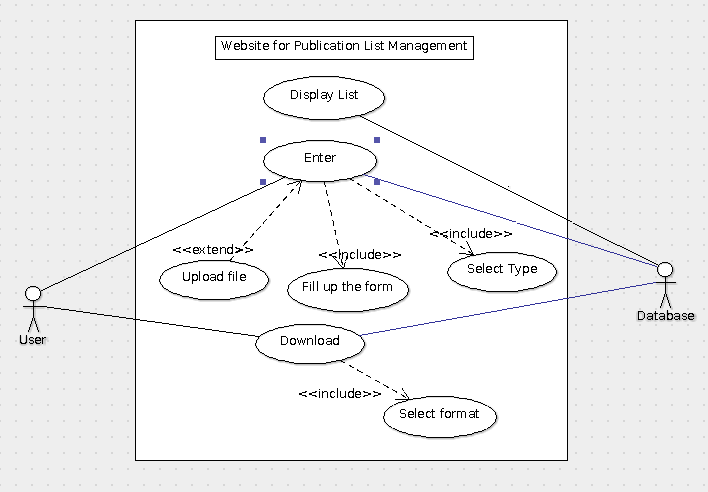
\includegraphics[scale=0.6]{funcreq}
	\subsection{Non Functional Requirements}
		The non functional requirements of this venture are :
		
		\begin{enumerate}
			
			
			\item Compatibility
\\
			a.The software is web based and should be compatible with all popular modern browsers in any operating system.
			
			\item Dependency on other parties
\\
			a.The software should behave well with other parties that it depends upon
\\
			b.The other parties may include, but may not be limited to software frameworks it uses, external databases and physical hardware.
			\item Efficiency 
\\
			a.The software should be optimized to consume reasonable load.
			
			\item Integrability 
\\
			a.The software should be able to integrate the necessary components seamlessly.
			
			\item Modifiability
\\
			a.The prototype of the software should be modifiable according to any reasonable claims made by the client.
			\item Operability
\\
			a.The system should be operable under normal circumstances without disruption
			
			
			\item Robustness
\\
			a.The system should be able to generate errors and should work accordingly in the case of various errors and erroneous inputs
			\item Security (cyber and physical) \\
			a.It should be secure so that hackers or any parties with malicious intent cannot retrieve or alter any confidential data
			\item Scalability 
\\
			a.The system should be able to handle growing number of users as well as growing data to the users
			\item Usability (Human Factors) \\ 
			a.The software and the underlying technology should be as intuitive and easy to use as possible from the perspective of a user
		\end{enumerate}
		
	\newpage
	\section{Analysis Models}
	\subsection{Context Model}
		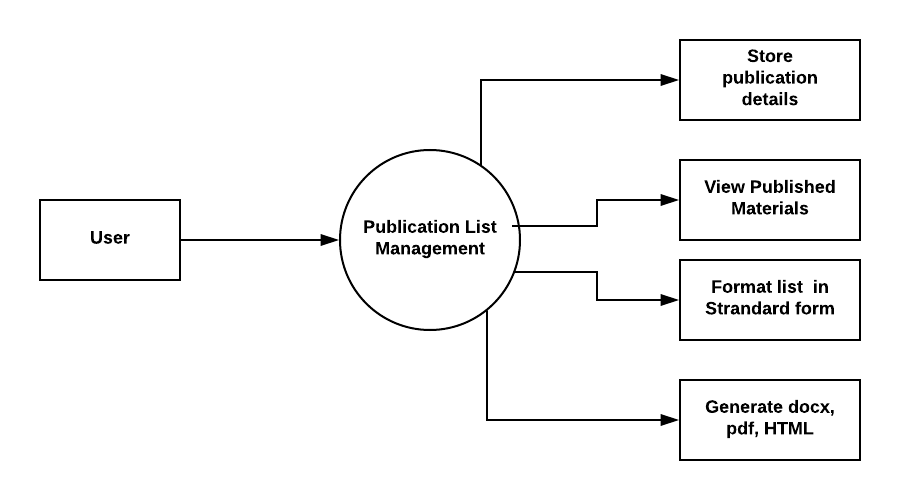
\includegraphics[angle=90, scale=1.7]{dfd0v2}
	\newpage
	\subsection{DFD}
		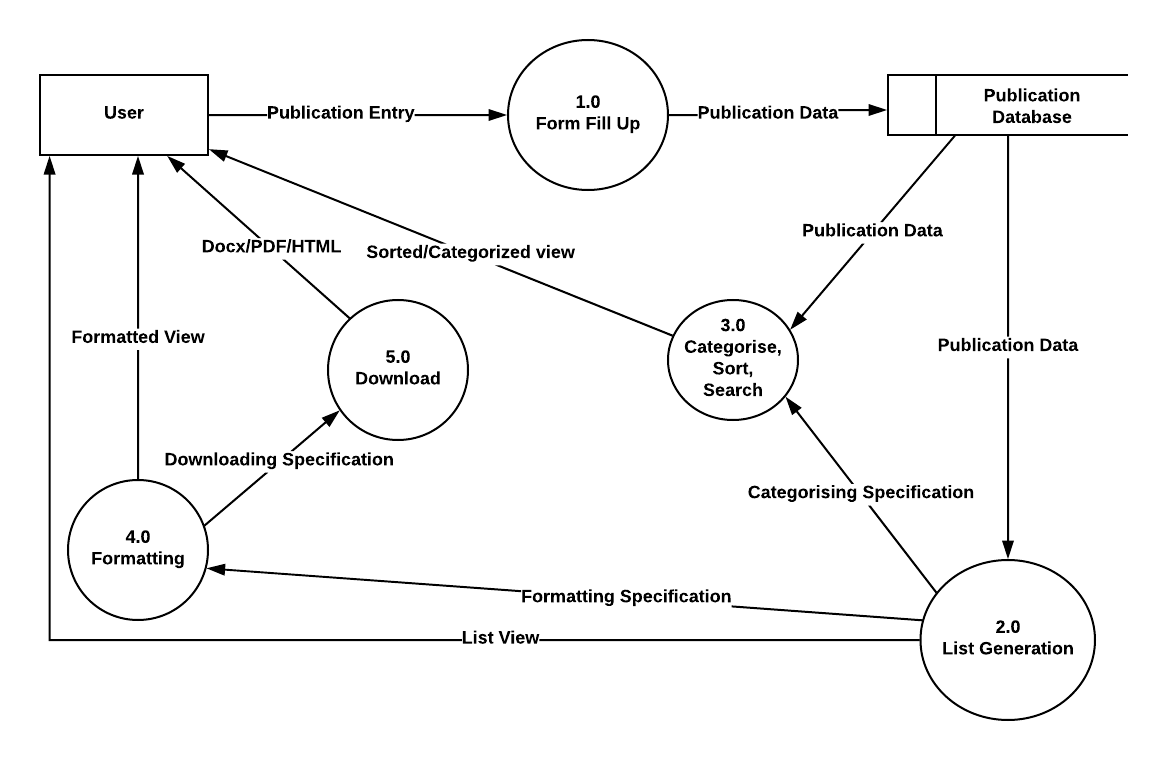
\includegraphics[angle=90, scale=1.3]{dfd1v2}
	\newpage
	\subsection{ERD}
		Entity Relationship Diagram: \\
		
			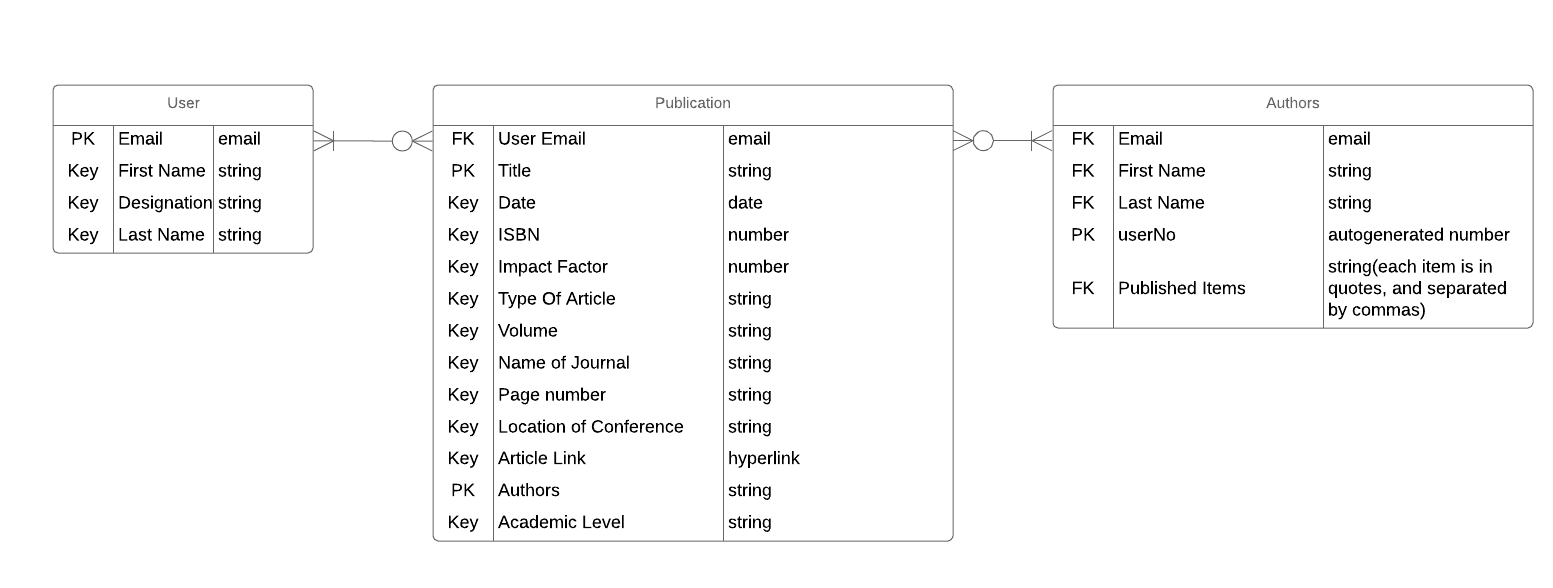
\includegraphics[angle=90, scale=1.8]{seq/erdv2}\\

	\subsection{Use Case Diagrams}
	
		\subsubsection{Use Case Diagram:}
			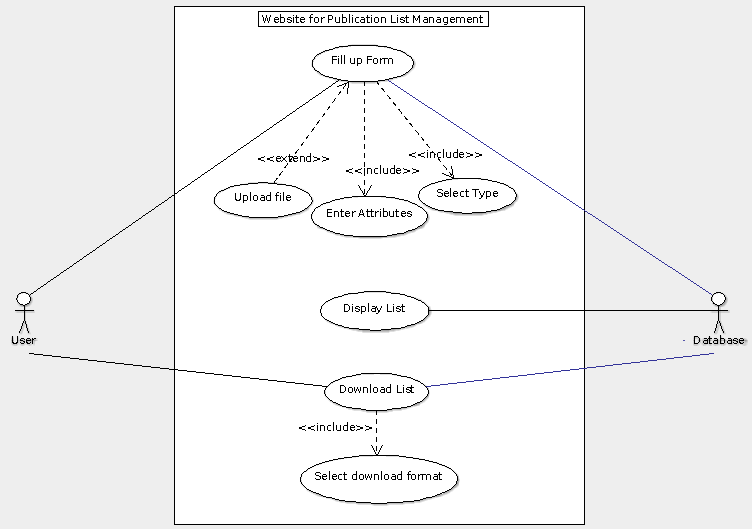
\includegraphics[scale=0.5]{UCD}
		\subsubsection{Fill Form Use case Diagram:}
			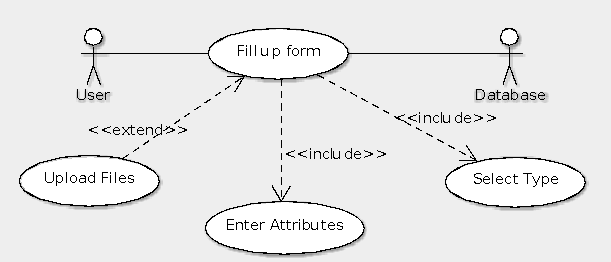
\includegraphics[scale=0.6]{uc/ffuc_diag}
			\\
			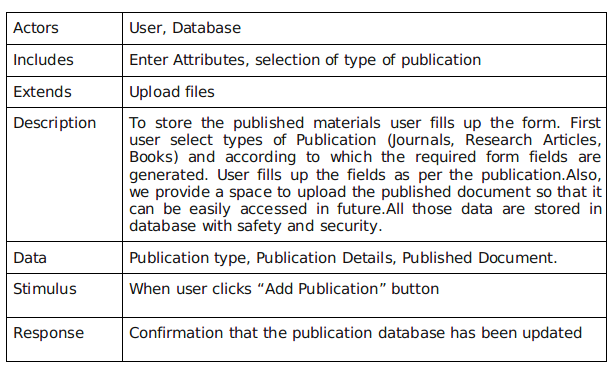
\includegraphics[scale=0.7]{uc/fillformusecase}
		\subsubsection{User in Use case Diagram:}
		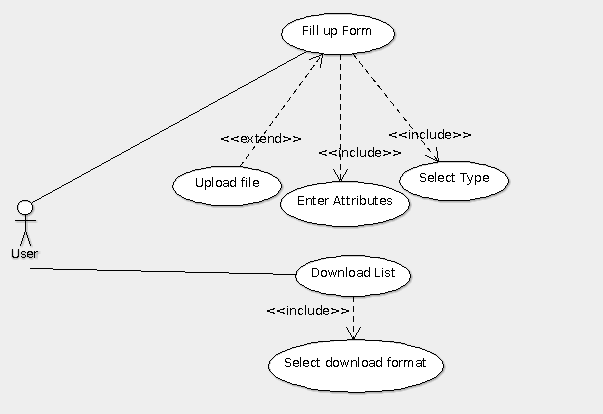
\includegraphics[scale=0.7]{User_in_UCD}\\
		User performs following activities:
		
		\begin{enumerate}
			\item Fill Up form: User selects the type of publication, fills up the generated fields and upload the published documents.
			\item Views the list and downloads the list: User selects the type of formatting to generate the list and type of file to download the formatted list.
			
			
			
		\end{enumerate}
		\subsubsection{Database in use case Diagram:}
		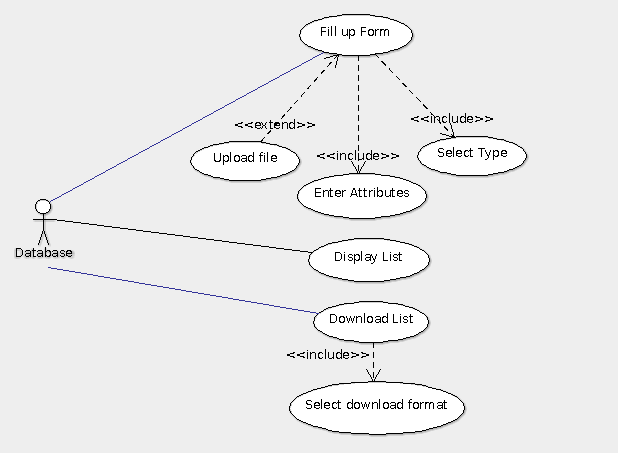
\includegraphics[scale=0.7]{Database_in_UCD}
		\\
		
		Database is associated in following activities:
		\begin{enumerate}
			\item Form fill up process to store attributes, data and files.
			\item Generation of List: Database provides the data to generate the list of published materials.
			\item Downloading list: Database provides the data to download the list.
			
		\end{enumerate}
		\subsubsection{Display List use case Diagram:}
		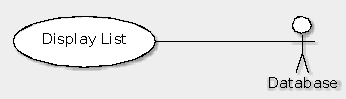
\includegraphics[scale=0.5]{Display_List_Use_Case}
		\\
		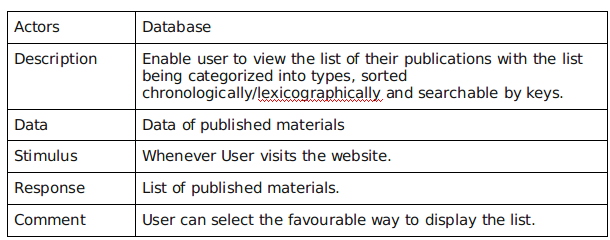
\includegraphics[scale=0.7]{uc/displaylistusecase}
		
		\subsubsection{Download List use case Diagram:}
		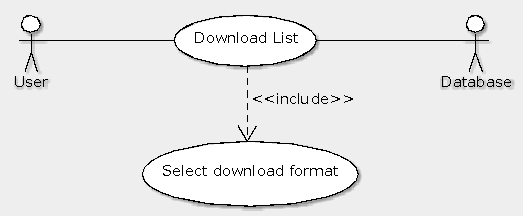
\includegraphics[scale=0.5]{Download_List_Use_Case}
		\\
		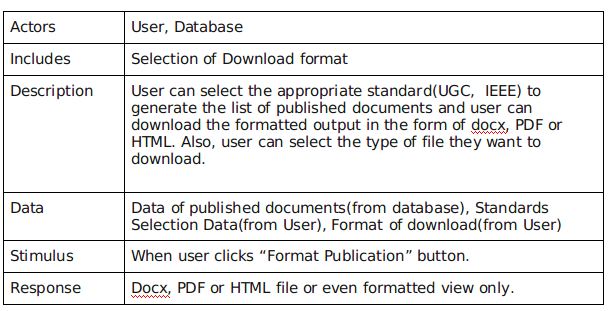
\includegraphics[scale=.7]{uc/downloadlistusecase}
	\newpage
	\subsection{Sequence Diagram}
		\subsubsection{Publication Entry:}
		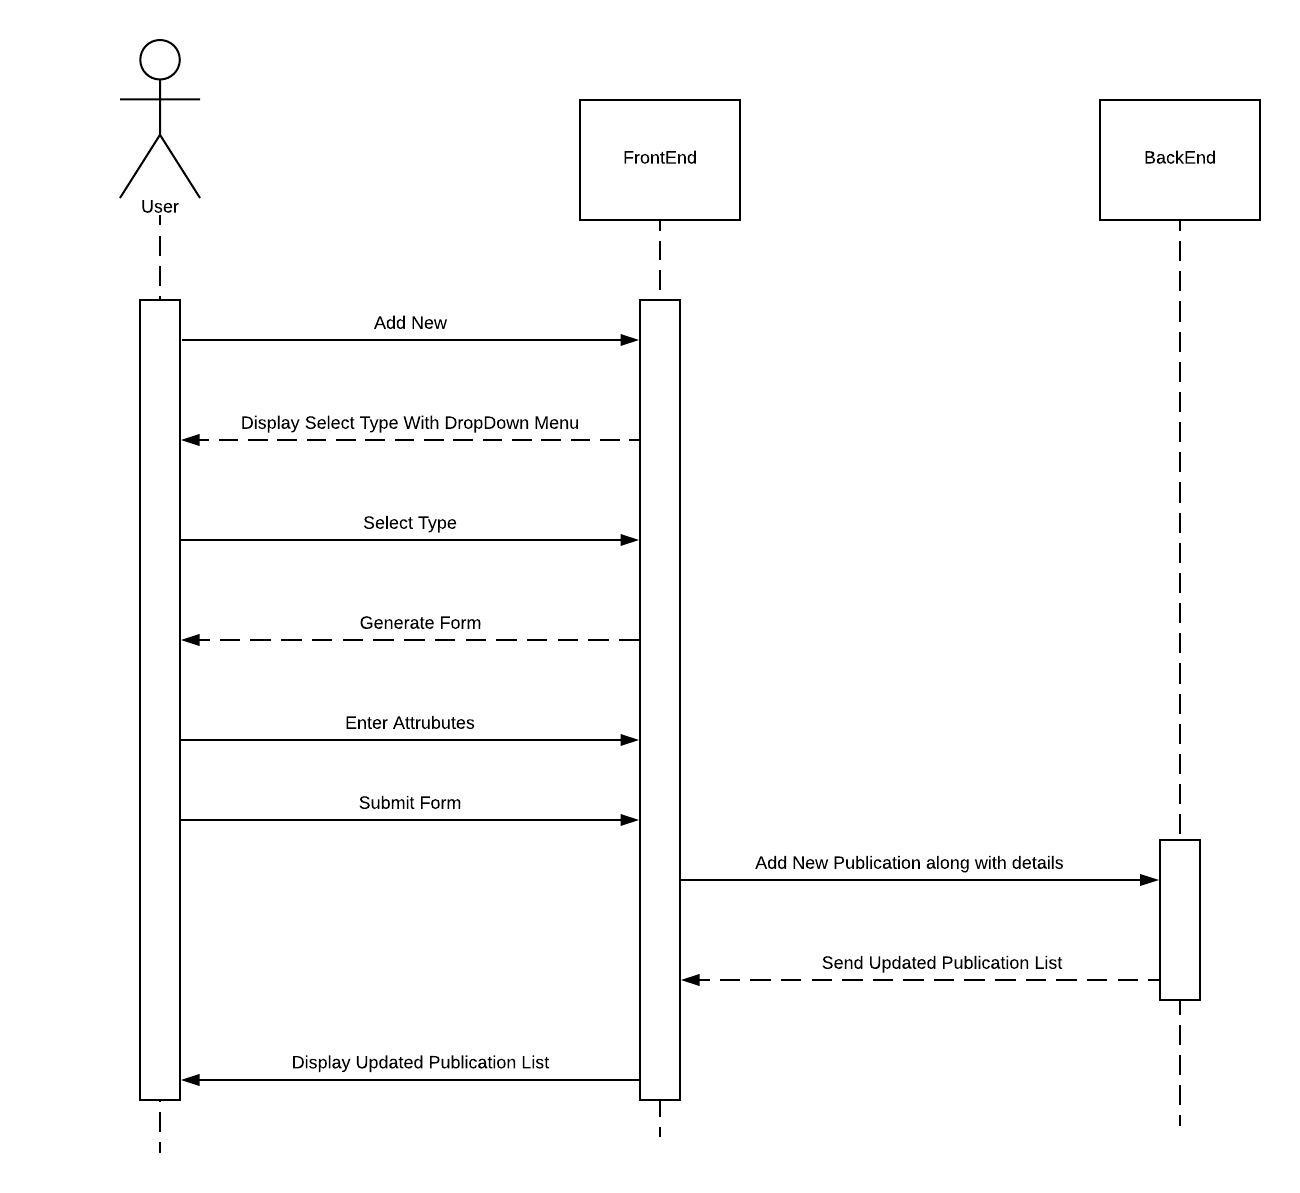
\includegraphics[scale=0.7]{seq/fill_form}
	
		\subsubsection{List Download }
		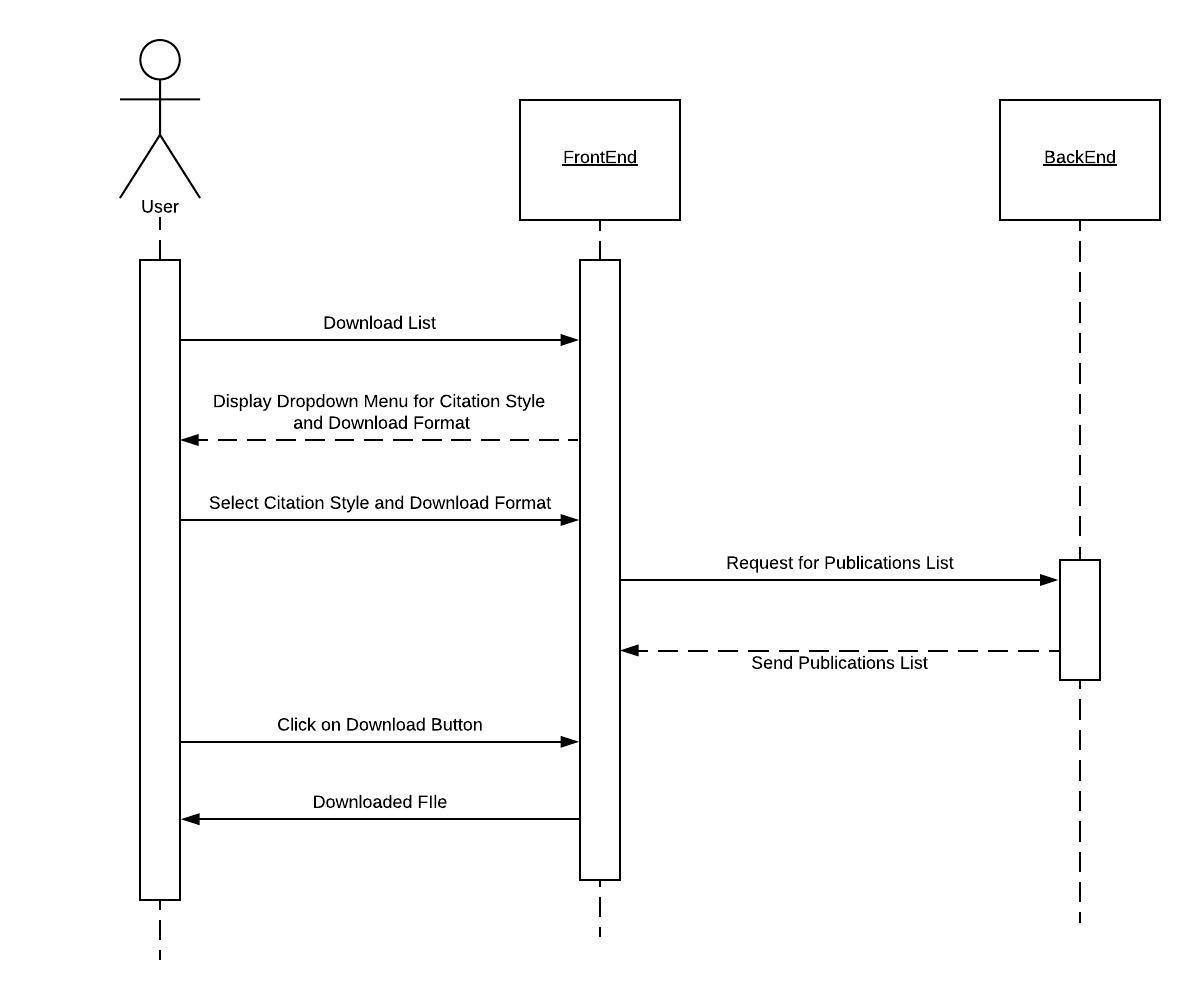
\includegraphics[scale=0.7]{seq/download_list}
		
		\subsubsection{Display list:}
		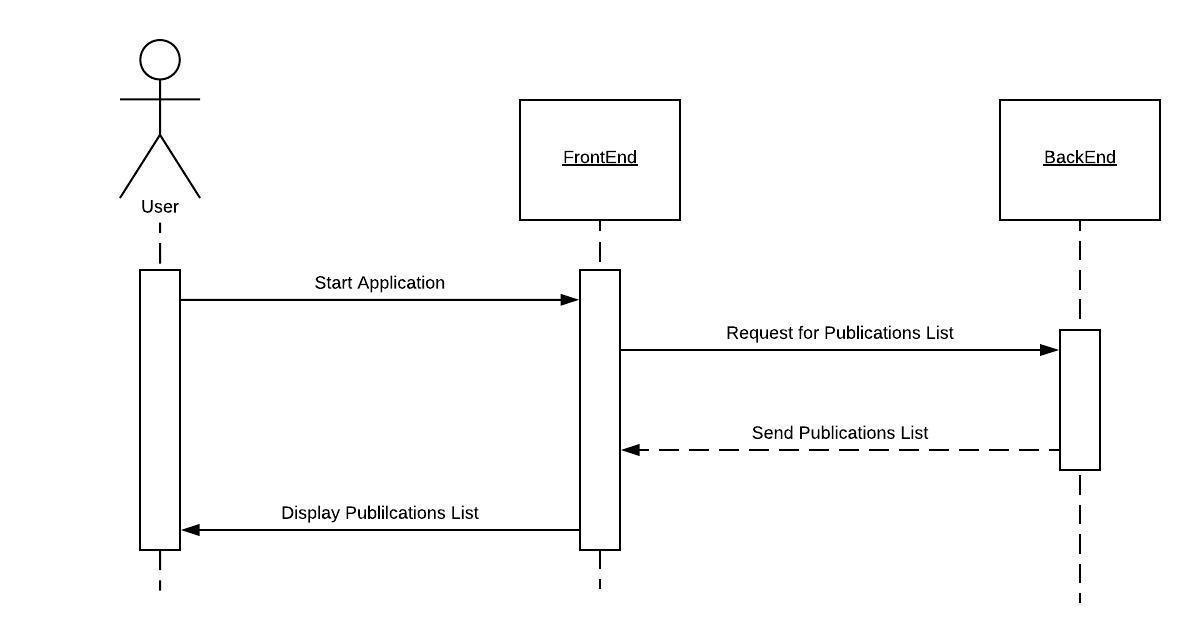
\includegraphics[scale=0.7]{seq/display_list}
		
		
	\newpage
	\subsection{Interface Design}
		\subsubsection{Main Interface / Homepage:}
			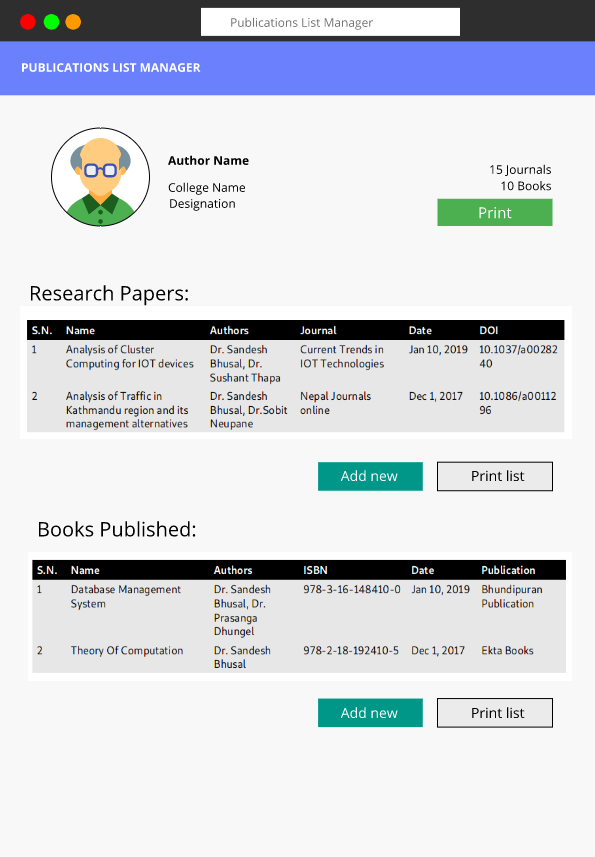
\includegraphics[scale=.7]{main_interface}
			
		\subsubsection{Print Format Selection Prompt:}
			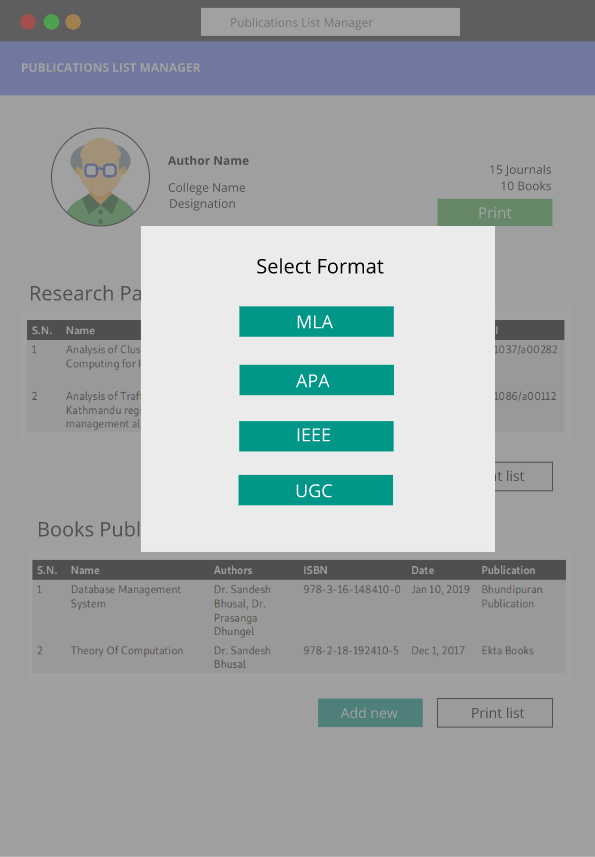
\includegraphics[scale=.7]{print_format_select}
		\subsubsection{Entry Interface:}
		\vspace{10mm}
			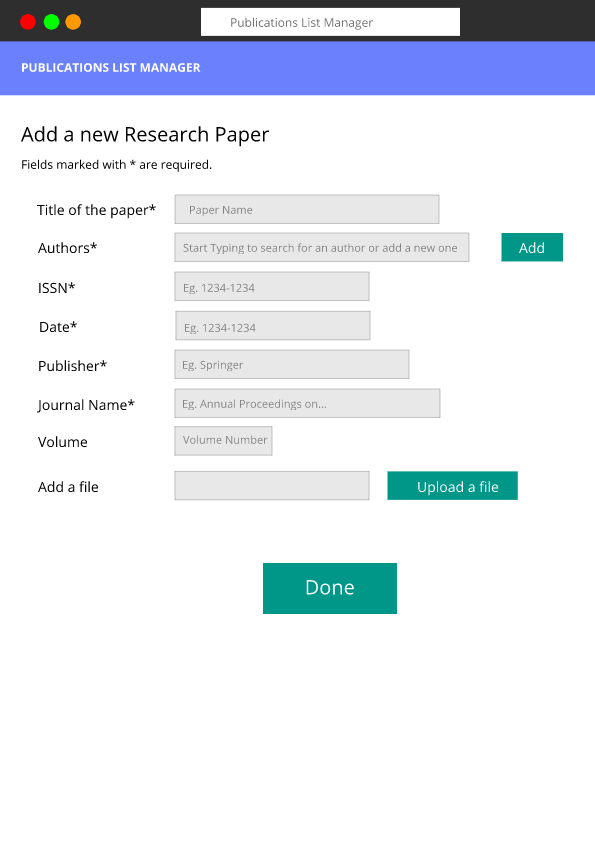
\includegraphics[scale=.7]{entry_form_interface}

\end{document}